\chapter{Analysis of Related Work}
\label{ch:related_work}
This chapter outlines previous work by other researchers that is relevant to this thesis, supplementing the background information provided in Ch.~\ref{ch:background}. A lot of work and research has been and is being done in the field of learning with games and game-like approaches, but for practical reasons (there is a lot of material) this chapter only summarizes what I've found to be most relevant. This primarily includes work on tutorial design and teaching computer-related tasks through games, but some other work is also included to add perspective.

\section{Tutorial Design}
\label{sec:tutorial_design_related}
Tutorials, as described in Sect.~\ref{sec:tutorials}, are widely used to teach users how to work with software products, among other things. With the tutorial, the creators aim to teach users how to perform various tasks with their tool, preferably in a \textbf{quick}, \textbf{intuitive}, \textbf{memorable}, and \textbf{error-free} way. Unfortunately, not all tutorial designs succeed in fulfilling all of these goals, but many efforts have been made to explore different approaches and improve on the standard tutorial design. Some of these are briefly described in the following sections.

\subsection{Stencils-Based Tutorials}
\label{sec:stencils}
The authors of the paper \emph{Stencils-Based Tutorials: Design and Evaluation}~\cite{kelleher:stencils} identify some problems with traditional tutorials: users may miss steps or perform actions that were not intended, and it is often difficult to find the components described in the tutorial.

\noindent
In their work, the authors introduce \emph{Stencils}, which is an alternative way of presenting a tutorial by adding a translucent colored interface layer on top of the original \gls{ui}, with holes highlighting the relevant elements, as seen in Fig.~\ref{fig:stencils}. Additionally, tutorial information is displayed on this layer in the form of sticky notes.

\begin{figure}[htp]
	\centering
	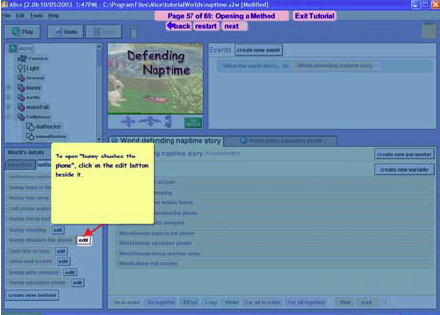
\includegraphics[width=0.8\textwidth]{stencils}
	\caption[\emph{Stencils} example]{An example of highlighting relevant \gls{ui} elements with \emph{Stencils} through holes in the colored layer. Tutorial information is added with the yellow sticky note. \emph{Image source:~\cite{kelleher:stencils}}}
	\label{fig:stencils}
\end{figure}

\noindent
With the results of a user study, the authors show that with a \emph{Stencils}-based tutorial, users were able to complete tutorials faster, with fewer errors and less human assistance. They also note that their tutorial approach can likely be improved by decreasing the level of assistance depending on the users familiarity with the system. A need for tutorial tasks that are directly relevant to the users, as opposed to ``artificial'' tutorial exercises, is also mentioned.


\subsection{DocWizards}
\label{sec:docwizards}
The authors of the paper \emph{DocWizards: A System for Authoring Follow-me Documentation Wizards}~\cite{bergman:docwizards} identify that there are some problems with teaching people to use software (\emph{computer-based procedures}) through documentation alone. Users must find \gls{ui} elements based on documentation descriptions on their own, understand and handle conditional branches, and at the same time keep track of where they are in the process.

\noindent
In their work, they propose the use of a tutorial-like documentation process called \emph{follow-me documentation wizards}, an approach that combines the advantages of conventional wizards and documentation. With their approach, processes are automatically captured from demonstrations made by expert users, and made available to new users in the form of highlighting both text from the documentation (see Fig.~\ref{fig:docwizards}) as well as UI elements for each step.

\begin{figure}[htp]
	\centering
	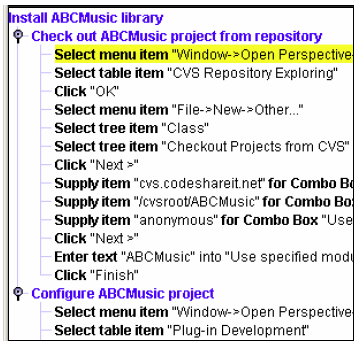
\includegraphics[width=0.6\textwidth]{docwizards}
	\caption[\emph{DocWizards} example]{An example of stepwise instructions in \emph{DocWizards}. The current step is highlighted in yellow. \emph{Image source:~\cite{bergman:docwizards}}}
	\label{fig:docwizards}
\end{figure}

\noindent
TODO: rewrite
Finally, a user study is conducted by the authors to evaluate their system, yielding positive results. The usefulness of the \emph{DocWizards} approach has also been verified in a separate study~\cite{gweon:evaluating_docwizards}.

\subsection{Graphstract}
\label{sec:graphstract}
The authors of the paper \emph{Graphstract: Minimal Graphical Help for Computers}~\cite{huang:graphstract} identify problems with the commonly used approach of providing only a textual explanations in software tutorials and help. Users are unlikely to read these explanations carefully enough, if at all. Simply adding screenshots of the \gls{ui} is not an adequate solution, since these usually add far more information than necessary, and thus increase the perceived size and complexity of the explanation. Problems with animation and video are also identified, such as making it difficult for the user to move at their own pace.

\noindent
Instead of relying on text-only descriptions or simple screenshots, the authors propose the use of graphical help in the form of partial screenshots, combined to show a complete sequence of actions required to perform a task (see Fig.~\ref{fig:graphstract}). This approach provides graphical help directly mapped to the \gls{ui}, without adding a lot of extra information. Additionally, the whole sequence is presented in a small space, making it easy to get an overview.

\begin{figure}[htp]
	\centering
	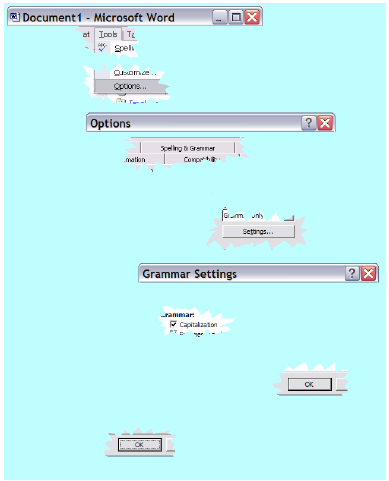
\includegraphics[width=0.7\textwidth]{graphstract}
	\caption[\emph{Graphstract} example]{An example of stepwise instructions in \emph{Graphstract} in the form of screenshot snippets, showing the steps required to toggle auto-capitalization in Microsoft Word. \emph{Image source:~\cite{huang:graphstract}}}
	\label{fig:graphstract}
\end{figure}

\noindent
Three iterations of user studies on a prototype is conducted by the authors, showing that \emph{Graphstract} performs better than conventional approaches overall, if not in all cases. They also conclude that adding text to the images is useful in many situations, despite their approach relying on graphical help only.

\subsection{Photo Tutorials}
\label{sec:photo_tutorials}
The authors of the paper \emph{Generating Photo Manipulation Tutorials by Demonstration}~\cite{grabler:photo_tutorials} argue the use of static visual tutorials (stepwise text-based tutorials accompanied by graphics) over video-tutorials for image processing software.

\noindent
In their work, the authors design a system for auto-generating static visual tutorials for a specific software product. These tutorials provide stepwise instructions with screenshots for completing a particular task, and additionally highlight the parts of the screenshots that are relevant to this task, as seen in Fig~\ref{fig:photo_tutorials}. This is combined with macros for automatic image labeling, to identify important regions of the particular image the user is working with.

\begin{figure}[htp]
	\centering
	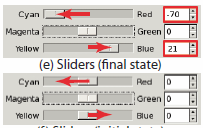
\includegraphics[width=0.5\textwidth]{photo_tutorials}
	\caption[\emph{Photo Tutorials} example]{An example of highlighting relevant \gls{ui} elements in a screenshot with \emph{Photo Tutorials}. \emph{Image source:~\cite{grabler:photo_tutorials}}}
	\label{fig:photo_tutorials}
\end{figure}

\noindent
Through a user study, the authors verify the effectiveness of their tutorials by observing that users perform significantly better and make less errors compared to tutorials based on text and video. However, some problem areas are identified: better tutorials can be created by providing feedback to users as they are performing the steps of the tutorial.

\subsection{Toolclips}
\label{sec:toolclips}
The authors of the paper \emph{ToolClips: An Investigation of Contextual
Video Assistance for Functionality Understanding}~\cite{grossman:toolclips} explore the \emph{learnability} of software products, more specifically relating to the concept of \emph{understanding} how to properly use functionality (see~\cite{grossman:software_learnability}). They identify problems with existing approaches based on both text and videos, where information is provided outside the context of the \gls{ui} in question. The authors also assess that regular tooltips, which provide the user with a short in-context description of what a \gls{ui} element does, do not provide a sufficient level of detail for complex tools.

\noindent
Attempting to provide the best of several worlds, the authors suggest their \emph{ToolClips} approach, enhancing regular tooltips with additional documentation and video content, in a more context-sensitive manner, as seen in Fig.~\ref{fig:toolclips}.

\begin{figure}[htp]
	\centering
	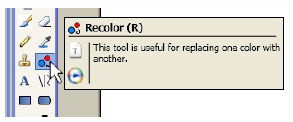
\includegraphics[width=0.7\textwidth]{toolclips}
	\caption[\emph{ToolClips} example]{An example of a \emph{ToolClip}, appearing as a regular tooltip, but with buttons allowing access to additional media. \emph{Image source:~\cite{grossman:toolclips}}}
	\label{fig:toolclips}
\end{figure}

\noindent
Through the results of two user studies, the authors show that the \emph{ToolClips} approach significantly improves users' understanding of how to use elements, and additionally has a positive impact on retention of this understanding, for applications that are \emph{highly graphical}.

\subsection{A Summary of Good Practices for Tutorials}
\label{sec:good_practices_tutorials}
The previous sections in this chapter, as well as Sect.~\ref{sec:tutorials}, describe various research efforts on the creation of good tutorials and introductions for computer-based procedures. Different aspects of the learning process are considered, and it is apparent that there are many ways to succeed. In this section, I attempt to summarize the various aspects that should be considered when making a tutorial for a computer-based procedure.

\paragraph{Interactivity and Active Learning} The most important aspect of a good tutorial is likely that it should be interactive. Active learning is one of Chickering and Gamson's \emph{seven principles of learning}~\cite{chickering:seven_principles}, in addition to being recommended for tutorial design by various other sources~\cite{bowerman:tutorial_design, aberson:tutorial_evaluation}. A common way of making a tutorial interactive is to provide exercises the user must complete.

\paragraph{Feedback} If a user is presented with tasks and exercises during the tutorial, it should also be possible to see the results of these exercises, and if applicable, check if the results are correct~\cite{chickering:seven_principles}. The feedback should also give the user some indication of the user's performance compared to the learning objectives~\cite{bowerman:tutorial_design}.

\paragraph{Motivation} It is important for users to know not only why they should learn the processes described in the tutorial (i.e. how these processes are useful to them), but also why they should complete more advanced tutorials on the subject that may optimize their work~\cite{grossman:software_learnability}. Users should also be informed of the scope of the tutorial, and what they are supposed to learn~\cite{bowerman:tutorial_design}.

\paragraph{Reasonable Teaching Order} If a tutorial teaches multiple concepts, a reasonable teaching order should be established, particularly if these concepts build on each other~\cite{bowerman:tutorial_design}. When deciding on a starting point, user' background must also be considered.

\paragraph{Context-sensitivity of Information} All new information presented in the tutorial should be provided at the point where it is actually needed, as opposed to being presented in an introduction part before the tutorial starts~\cite{andersen:tutorials_impact}.

\paragraph{Visual Mapping of UI Elements} If \gls{ui} elements are referenced in the textual part of a tutorial, it should be easy to map these references to the actual \gls{ui}. This can be done by adding (partial) screenshots of the \gls{ui}~\cite{huang:graphstract}, or highlighting the elements that are relevant for the current step~\cite{kelleher:stencils, bergman:docwizards, grabler:photo_tutorials}.

\paragraph{Multimedia Content} A tutorial that consists of text alone is rarely adequate, and can be improved by adding multimedia content such as images, sound, or video~\cite{grossman:software_learnability}. This kind of multimedia information content can also be present in the application itself, providing the user with more resources when help is needed~\cite{grossman:toolclips}. Animations can also be advantageous, but should be used only where natural, for example to describe events in time~\cite{morrison:animation}.

\paragraph{Help-on-demand} While the user generally shouldn't have to read through too much text before starting the interactive part of the tutorial, additional information resources should be available for when the user gets stuck, or for other reasons needs to know more about a specific topic~\cite{andersen:tutorials_impact, grossman:toolclips}.

\paragraph{Relevant Tasks} When a tutorial contains tasks and exercises, these should be as relevant as possible to the user, as opposed to fictional tasks created only for learning purposes~\cite{kelleher:stencils}.

\paragraph{High Expectations} Users should be presented with high expectations from the beginning, so that they are prepared to make an effort in understanding the concepts taught by the tutorial~\cite{chickering:seven_principles}.

\paragraph{Address Misconceptions} If common misconceptions exist within the topic that is being taught, the tutorial should do its best to address these misconceptions, preferably before they even have a chance to form~\cite{aberson:tutorial_evaluation}.

\paragraph{Multiple Perspectives} Generally, we want the user to actually think reflectively about the topic being taught, and not just passively absorb the facts. One way of doing this is by offering multiple perspectives of various concepts~\cite{aberson:tutorial_evaluation}.

\paragraph{Freedom} When introducing something like a game or a software product through a tutorial, we have to consider the amount of freedom users are given in the tutorial. There are issues in both allowing users complete freedom to explore, and restricting them to a single path~\cite{andersen:tutorials_impact, bonawitz:double_edged_pedagogy}. The optimal solution likely lies somewhere in between, by for example offering \emph{directed exploration}~\cite{esper:codespells}. 

\section{Learning With Games}
\label{sec:learning_with_games}
Most video games require the player to learn something in order to complete the game, whether it is difficult concepts like solving obscure puzzles, or simply the controls of the game. In some cases, games are even used to teach concepts for educational purposes, such as programming. In other cases, games even teach players valuable real-life skills without being deliberately designed to do so. The following sections briefly describe some of the efforts previously made in the field of educational games.

\subsection{Karel the Robot}
\label{sec:karel_the_robot}
Karel the Robot~\cite{pattis:karel_the_robot} is a game-like programming language and environment designed to teach basic programming concepts to beginners. It was developed by Richard E. Pattis in 1981, who used Karel to teach programming courses at Stanford University.

\noindent
The motivation behind Karel was to be able to teach students the basics programming without having to worry about the more complex and less important (to beginners) details. In Pattis' own words: \emph{``The careful omission of variables and data structures from Karel's language ... allows the immediate exploration of the rich domain of abstraction and control structures.''}~\cite{pattis:karel_the_robot}. This allows students to focus on learning how to solve problems through programming concepts.

\noindent
Karel was originally designed as a Pascal-like procedural programming language, but the concept gained wide popularity, and has been extended to Java~\cite{roberts:karel_the_robot_java},
Python,\footnote{\href{http://gvr.sourceforge.net/}{The Guido van Robot
Programming Language (link)}}$^{,}$\footnote{\href{https://code.google.com/p/rur-ple/}{rur-ple: an environment designed to help you learn computer programming using the language Python (link)}} Karel++ (object-orientation)~\cite{bergin:karel_plus_plus}, REALbasic,\footnote{\href{https://code.google.com/p/rbstuff/wiki/rbKarelOverview}{rbKarel:
REALbasic adaption of Karel the Robot (link)}} and Scratch.\footnote{\href{http://scratched.media.mit.edu/resources/karel-robot-scratch}{Karel the Robot in Scratch (link)}} Karel was inspired by the LOGO project,\footnote{\href{http://el.media.mit.edu/logo-foundation/index.html}{LOGO Foundation website (link)}} and has in turn inspired games like RoboMind\footnote{\href{http://www.robomind.net/en/index.html}{RoboMind website (link)}} and C-Sheep~\cite{anderson:c-sheep}.

\noindent
The purpose of the game is to control a robot (Karel) by giving it a set of commands, and perform tasks. Initially, only a small set of commands are available, but as part of the learning process, users must learn how to extend these commands. The simplest task Karel is asked to perform is to pick up a beeper, seen as the diamond shape in Fig.~\ref{fig:karel_the_robot}.

\begin{figure}[htp]
	\centering
	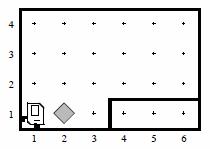
\includegraphics[scale=0.80]{karel_the_robot}
	\caption[Karel the Robot]{A simple \emph{Karel the Robot} level, where Karel (bottom left) must move to and pick up a single beeper (diamond shape). \emph{Image source:~\cite{roberts:karel_the_robot_java}}}
	\label{fig:karel_the_robot}
\end{figure}

\noindent
Karel the Robot has now been around for more than 30 years, and the teaching paradigm described has proved successful in introducing students to the art of programming.\footnote{See for example~\cite{krause:computer_science_air_force},~\cite{untch:karel_conventional_language},~\cite{becker:teaching_with_karel}} Students are allowed to explore advanced concepts in a safe environment with less relevant complexities removed, and in a way that makes them \emph{want} to learn. The concept has been adapted and refined in many ways over the years, but the core paradigm remains.

\subsection{Josef the Robot}
\label{sec:josef_the_robot}
Josef the Robot~\cite{tomek:josef_the_robot} is a game-like programming environment similar to Karel (Sect.~\ref{sec:karel_the_robot}). Unlike Karel, Josef more closely resembles ``real'' programming languages by being rich in structures and operations. Like Karel, Josef is also inspired by the LOGO project.

\noindent
The author of Josef, Ivan Tomek, provides ample motivation for creating a more novice-friendly environment for learning how to program. Firstly, potential learners should find the problems they can solve with programming to be interesting, which is likely not the case (for the average person) with problems like sorting a sequence of numbers. Furthermore, novice programmers should not have to worry about the more complex rules that are not directly related to problem-solving, such as syntax and data handling.

\subsection{Serious and Epistemic Games}
\label{sec:serious_games}
Games that are designed for a purpose that is not pure entertainment are often called \emph{Serious Games}, a term likely popularized by \emph{The Serious Games Initiative}\footnote{\href{http://www.seriousgames.org/}{The Serious Games Initiative website (link)}} in 2002~\cite{djaouti:serious_games_origins}. This genre encompasses many different types of games, but a prime example of a serious game is the \emph{flight simulator}, a realistic type of game that exists in various forms, and is extensively used to teach pilots how to fly aircraft.

\noindent
The idea behind serious games is to improve student motivation and engagement by providing immersive learning experiences, similar to how many professions are taught. I can read a lot about woodworking, but in order to become a good carpenter, I must practice. Seeing actual results of my knowledge and skills in woodworking is also likely to be more enjoyable than simply imagining how it might look. Games can provide a similar kind of (simulated) hands-on experience for topics that are difficult or inconvenient to practice immersively, especially more abstract topics like math or computer programming, and this has also proved to be a more efficient learning method in many cases. Children especially learn and are better motivated by the kind of problem-solving we find in games, as opposed to traditional textbook learning~\cite{freitas:serious_games_new_paradigm}.

\noindent
Several organizations working with serious games exist. Some examples are the \emph{Serious Games Institute},\footnote{\href{http://www.seriousgamesinstitute.co.uk/}{Serious Games Institute website (link)}} the \emph{Games Learning Society},\footnote{\href{http://www.gameslearningsociety.org/}{Games Learning Society website (link)}} the \emph{Learning Games Network},\footnote{\href{http://learninggamesnetwork.org/}{Learning Games Network website (link)}} and \emph{Serious Games Interactive}.\footnote{\href{http://www.seriousgames.net/}{Serious Games Interactive website (link)}} These represent both commercial, societal, and academic interest in serious games.

\noindent
Researchers at the University of Wisconsin coined the term \emph{Epistemic Games} for the subset of serious games that aim to teach specific professions or skills~\cite{shaffer:epistemic_games}. They argue that games can help teach students to apply their knowledge, instead of simply remembering, in addition to facilitate for \emph{innovative} learning. With this as a basis, \emph{The Games and Professional Simulations Research Consortium}\footnote{\href{http://edgaps.org/gaps/}{The Games and Professional Simulations Research Consortium website (link)}} has been formed in order to solve educational challenges through games and simulations.

\subsection{CodeSpells}
\label{sec:codespells}
\emph{CodeSpells} is a project from the University of California, San Diego, that aims to teach Java programming through a wizardry game~\cite{esper:codespells}. The CodeSpells team draws inspiration from the \emph{epistemic games} concept, and their games immerses novice programmers in a world that connects abstract code (Fig.~\ref{fig:codespells_spell}) with visual and ``physical'' effects in the environment (Fig.~\ref{fig:codespells_fire}).

\begin{figure}[htp]
	\centering
	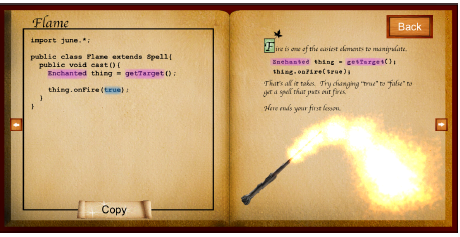
\includegraphics[scale=0.80]{codespells_spell}
	\caption[Java code for a CodeSpells spell]{An example of the CodeSpells spellbook, with Java code for the \emph{Flame} spell. The second page adds a short description, and a tip on how the spell can be modified. \emph{Image source:~\cite{esper:codespells}}}
	\label{fig:codespells_spell}
\end{figure}

\begin{figure}[htp]
	\centering
	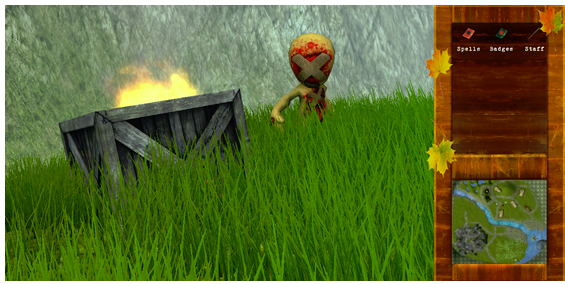
\includegraphics[scale=0.80]{codespells_fire}
	\caption[The CodeSpells game environment]{The game environment presented to the user in \emph{CodeSpells}. In this particular quest, the player must modify the \emph{Flame} spell (Fig.~\ref{fig:codespells_spell}) in order to extinguish the fire by setting \emph{thing.onFire(false)}. Image source: \emph{\url{https://sites.google.com/a/eng.ucsd.edu/codespells/home/level-1-quests}}}
	\label{fig:codespells_fire}
\end{figure}

\noindent
An important goal for the CodeSpells project is for students to gain a deep understanding of the programming language they use and problems they solve, and retain this understanding after completing the game. They would also like the students to be able to play the game without instructor assistance, and have focused extensively on designing quests that provide the appropriate scaffolding, as well as encourage exploration beyond the minimum required to move on~\cite{esper:design_quests_java_concepts}.

\noindent
In order to verify and improve the usefulness of their game for teaching programming, the CodeSpells team have conducted some user studies. Through these studies, they discovered that by immersing users in the game, the users developed a determination and a positive outlook on solving programming challenges~\cite{esper:codespells}. The team also discovered some principles that can be used to improve quest design~\cite{esper:design_quests_java_concepts}:

\begin{itemize}
	\item Provide examples that can be tested and used as a starting point, allowing users to see their effects.
	\item While the introduction should make it possible to perform complex actions with little effort, expectations for more effort should be provided from the beginning, letting users know that they have to build on and modify the examples.
	\item Provide directed exploration through quests, so the user can get a sense of complexity ordering and a choice of which challenge to overcome.
\end{itemize}

\noindent
These principles can likely also be used to improve design of other serious games.

\subsection{Non-Serious Games}
\label{sec:non-serious_games}
While the term \emph{Serious Games} covers the type of games that are designed for purposes other than entertainment, there are many examples of games designed for entertainment that ``accidentally'' teach their players valuable skills and knowledge.

\noindent
James P. Gee is a famous advocate for game-based learning. Through his analysis of various ``non-serious'' games, he identifies good principles of learning present in many of these games~\cite{gee:learning_machines}:

\begin{itemize}
	\item{\textbf{Empowered Learners:}} Players feel like active agents while playing, and not just passive recipients of information. Games are interactive, which leads to perceived ownership and engaged participation.
	\item{\textbf{Customization:}} Players are in many cases allowed to make choices about how to play, such as adjusting difficulty or playing style. People are different, and learn in different ways.
	\item{\textbf{Identity:}} Players often take on new identities within the game, in which they become heavily invested. This leads to a level of commitment that facilitates for deep learning.
	\item{\textbf{Manipulation and Distributed Knowledge:}} When players are able to control and manipulate a character or an object in the game environment, they feel expanded and empowered. Often, part of the knowledge required for manipulation is stored in the game itself (automated), so that the player can focus on the parts that are important for their task (and ``level of abstraction'').
	\item{\textbf{Well-ordered Problems:}} Players are exposed to problems in a well-ordered manner, so that they can form hypotheses that not only work in the moment, but prepare them for more difficult challenges later in the game.
	\item{\textbf{Pleasant Frustration:}} Players are exposed to problems that are neither too easy or too hard, but at the edge of the players' competence, and at their own pace.
	\item{\textbf{Cycles of Expertise:}} Players are allowed to repeat and practice skills until they become nearly automatic. Then, as the game progresses, they might have to adapt their skills to new conditions, and repeat the cycle.
	\item{\textbf{Context-sensitivity of Information:}} Players are often presented with the information they need \emph{when} they need it, instead of having to memorize it in advance.
	\item{\textbf{Fish Tanks:}} In many cases, games serve as simplified versions of real-world systems, and illustrate some important concepts while hiding complexities that might be too difficult to handle for novices. Sometimes, such fish tanks are also created within the game itself, in the form of tutorials. This allows players to exercise their skills without having to worry about \emph{all} the details.
	\item{\textbf{Sandboxes:}} Games also provide a safe environment for exercising skills, where the cost of failure generally is low compared to the real world.
	\item{\textbf{Skills as Strategies:}} Instead of practicing for the sole purpose of becoming good, players see the skills they learn as a strategy towards accomplishing goals within the game. This provides better motivation by allowing ``in-context'' practice.
	\item{\textbf{System Thinking:}} Many games consist of smaller elements, where players must understand how all the elements interact fit into the overall system of the game.
	\item{\textbf{Meaning as Action Image:}} Instead of just providing definitions and descriptions, games present concepts through visualizations and experiences, which is closer to how people actually think.
\end{itemize}

\noindent
These are clearly principles that should be considered also in serious and educational games, not only those made for entertainment. As Gee points out, \emph{``When we think of games, we think of fun. When we think of learning, we think of work''}. If done right, it is likely possible to merge the tedious process of learning with the fun of games with equal or better results.

\subsection{A Summary of Good Practices for Educational Games}
\label{sec:good_practices_games}
While educational games by default generally incorporate some good learning practices (interactivity and feedback), some ways of designing and implementing such a game are likely better than other. Based on the work described in the previous sections as well as Sect.~\ref{sec:game_based_learning}, this section summarizes some additional aspects that should be considered when designing an educational game.

\paragraph{Tutorials} Many games start by guiding the player through a tutorial in order to learn the basics of the game, which is similar to completing a tutorial in order to learn about a topic like programming language. Games, particularly complex ones, may benefit from having a tutorial introduction, in the form of increased player engagement~\cite{andersen:tutorials_impact}. Since educational games are often used to teach complex concepts, creating a tutorial is generally justified. The principles listed in Sect.~\ref{sec:good_practices_tutorials} also apply to tutorials for educational games, since these should be at least as good as tutorials for teaching a specific topic. Because of their immersive nature, video games likely makes a some of these principles easier to follow, such as providing good visual mapping of \gls{ui} elements and suitable multimedia content.

\paragraph{Immersion} By providing an \emph{immersive} experience, educational games can provide better motivation and encouragement for players to interact with and explore the concepts taught~\cite{esper:codespells}. Providing an immersive experience may include giving the player a sense of \emph{identity} in the game, enhancing commitment, or provide \emph{fish tanks} or \emph{sandboxes} where players can discover, explore, and experiment with concepts in safe and possibly simplified environments~\cite{gee:learning_machines}. Immersive game experiences also provide players with meaning for verbal concepts, through visualizations and experiences~\cite{gee:learning_machines}.

\paragraph{Exploration and Guidance} The discussion of exploration versus guidance becomes even more important for educational games than for tutorials. Good educational games often provide a safe environment where concepts can be explored and experimented with, even without any guidance. In many cases, too much guidance may even prevent exploration and discovery to some degree~\cite{bonawitz:double_edged_pedagogy}. Depending on the complexity of the concepts taught, having no guidance at all is also not a good solution. Some players will have more trouble than others understanding certain concepts, and subtleties are not always intuitively understood. The optimal solution is to evaluate the game's complexity, and provide some kind of middle ground (directed exploration,~\cite{esper:design_quests_java_concepts}) tailored not only to how difficult the concepts are, but the player's previous knowledge and ability to understand them. Users may even be allowed to choose their own difficulty level based on their own perceived experience level and skill.

\paragraph{Simplicity and Challenge} Irrespective of their background, any users within the target audience should be able to get started and see results early in the introduction~\cite{esper:design_quests_java_concepts}. However, the problems presented must eventually become difficult enough to allow players to gain deep understanding of the concepts taught, and expectations of this should be present from the beginning. Additionally, players can progressively be presented with an environment that is more and more like a real environment. This can help make the transition from practicing skills in a video game, to using these skills in real situations smoother~\cite{untch:karel_conventional_language}.
